\documentclass{standalone}
\usepackage{pgfplots}
\usepgfplotslibrary{polar,fillbetween}
\newcommand*{\maximum}{26}
\begin{document}
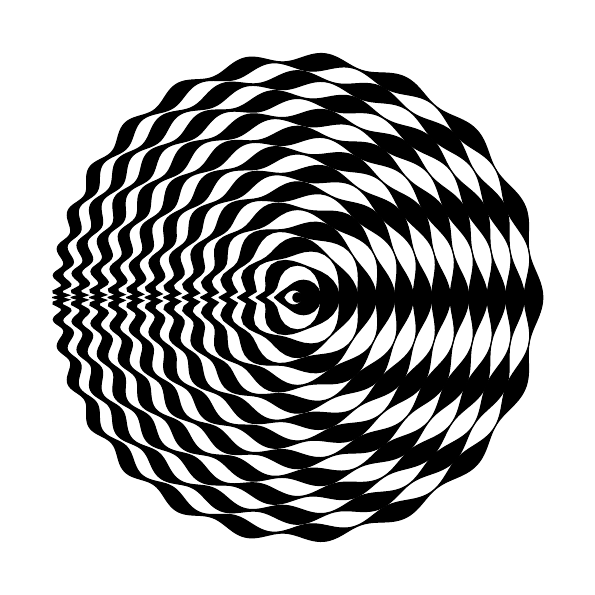
\begin{tikzpicture}
  \begin{polaraxis}[hide axis]
    \pgfplotsinvokeforeach{0,...,\maximum}{
      \pgfmathparse{20+#1^2}
      \pgfplotsset{samples=\pgfmathresult}
      \addplot[name path = #1, mark=none, solid, domain=0:360]
        { -(#1*2 + cos(#1*2*acos(x/180-1))) }; }
    \addplot[name path=-1] coordinates {(0,0)};% Startbezug filling
    \foreach \i [evaluate=\i as \j using int(\i-1)] in {0,2,...,\maximum}{
        \edef\temp{[black] fill between[of=\i\space and \j]}
        \expandafter\addplot\temp;
    }
	\end{polaraxis}
\end{tikzpicture}
\end{document}